%-----------------------------------------------------------------------------
%	 Marco Aplicativo
%-----------------------------------------------------------------------------

\lhead[\thepage]{Metodología General de Trabajo \thechapter. \rightmark}
\rhead[Metodología General de Trabajo \leftmark]{\thepage}
\part{Marco Aplicativo}
%	Capitulo 6: Metodología General de Trabajo
\chapter{Metodología General de Trabajo}
\markboth{Metodología General de Trabajo}{Metodología General de Trabajo}

\section{Scrum}
\lhead[\thepage]{\thesection. Scrum}
Scrum es una metodología ágil y flexible para gestionar el desarrollo de software. Se basa en construir primero la funcionalidad de mayor valor para el cliente y en los principios de inspección continua, adaptación, auto-gestión e innovación.\cite{scrumsofteng} En Scrum se aplican de manera regular un conjunto de buenas prácticas para trabajar colaborativamente y obtener el mejor resultado posible de un proyecto.\\

Es parte de la filosofía de Scrum el poder realizar entregas parciales y regulares del producto final, priorizadas por el beneficio que aportan al receptor del proyecto. Por ello, Scrum está especialmente indicado para proyectos en entornos complejos, donde se necesita obtener resultados rápidamente, con requisitos son cambiantes o poco definidos, donde la innovación, la competitividad, la flexibilidad y la productividad son fundamentales.\\

En Scrum un proyecto se ejecuta en bloques temporales cortos y fijos (iteraciones que normalmente son de 2 semanas, aunque en algunos equipos son de 3 y hasta 4 semanas, límite máximo de feedback y reflexión). Cada iteración tiene que proporcionar un resultado completo, un incremento de producto final que sea susceptible de ser entregado con el mínimo esfuerzo al cliente cuando lo solicite. El proceso parte de la lista de objetivos/requisitos priorizada del producto, que actúa como plan del proyecto. En esta lista el cliente prioriza los objetivos balanceando el valor que le aportan respecto a su coste y quedan repartidos en iteraciones y entregas.\\  

La actividades que se llevan a cabo bajo la metodología de Scrum son las siguientes:

\begin{enumerate}
\item Planificación de la iteración: En el primer día de cada iteración, el equipo realza una reunión de planificación de la iteración. Esta etapa consiste en una primera fase de selección de requisitos, en la cual el cliente presenta al equipo la lista de requisitos priorizada del proyecto y se responden a las dudas que surgen sobre el dominio de las tareas a realizar y una segunda fase de planificación de la iteración, donde el equipo elabora la listas de tareas necesarias para desarrollar lo que se es requerido para la iteración, ademas de la estimación de esfuerzos por parte de los miembros del equipo.
\item Ejecución de la iteración: Cada día se realiza una reunión con todo el equipo de 15 minutos como máximo para inspeccionar el avance en la realización de las tareas, dependencias u actividades bloqueantes ye insumos pendientes para su culminación. Durante la iteración el Scrum Master (facilitador) se encarga de que el equipo pueda articularse y cumplir los compromisos adquiridos por el equipo.
\item Inspección y adaptación: El ultimo día de la iteración se realiza la reunión de revisión de la iteración. Esta se conforma de dos partes, la demostración en donde el equipo presenta al cliente el/los entregable(s) con los requisitos mínimos acordados y la retrospectiva en la que el equipo analiza si su manera de trabajar ha sido la adecuada, los problemas que han surgido, su solución, de forma que se pueda mejorar de manera continua la productividad.
\end{enumerate}

\section{Control de Versiones de Software}
\lhead[\thepage]{\thesection. Control de Versiones de Software}
Un software de control de versiones es un aquel que permite registrar y gestionar cambios a nivel del código fuente de manera histórica permitiendo retornar a versiones anteriores o comprar diferencias entre ellas.

Esto permite tener:
\begin{itemize}
\item Flujos de trabajo organizados:
\item Descripción de versiones:
\item Colaboración:
\item Historial de cambios: 
\end{itemize}

\subsection{Git}
Git es un sistema de control de versiones moderno, distribuido y seguro que fue desarrollado originalmente por Linus Torvalds en el año 2005. 

Entre sus características principales se destacan:
\begin{itemize}
\item Arquitectura distribuida:
\item Flexibilidad:
\item Seguridad:
\item Rendimiento:
\end{itemize}

\subsubsection{Git-Flow}
Git Flow es una metodología para usar Git en la que se combina ramas de función y ramas principales. Fue popularizado por Vincent Driessen en 2010. Los aspectos clave del modelo Git Flow son:
\begin{itemize}
\item Ramas principales y de desarrollo: En lugar de tener una única rama principal, Git Flow utiliza dos ramas principales:
\begin{enumerate}
\item Main (o Master): Almacena el historial oficial de publicación.
\item Develop: Sirve como rama de integración para las funciones.
\end{enumerate}
\item Ramas de función: Los desarrolladores crean ramas de función para trabajar en características específicas. Estas ramas se fusionan con develop cuando la función está completa.
\item Ramas de publicación y corrección de errores:
\begin{enumerate}
\item Release Branches: Se crean a partir de develop para preparar una nueva versión. Aquí se realizan pruebas finales y se corrigen errores antes de la publicación.
\item Hotfix Branches: Se utilizan para corregir errores críticos en la versión actual de producción. Se crean a partir de main y se fusionan tanto con main como con develop.
\item Versionado y etiquetado: Git Flow simplifica la gestión de versiones al asignar números de versión a las confirmaciones en main y etiquetarlas.
\end{enumerate}
\end{itemize}

\section{Herramientas de Desarrollo}
\lhead[\thepage]{\thesection. Herramientas de Desarrollo}
A continuación se detalla aquellas herramientas de hardware y de software utiizados durante el desarrollo de este trabajo de investigación.

\subsection{Herramientas de Hardware}
Dado el enfoque de tener un grupo de dispositivos IoT que pudiesen obtener data real del entorno en donde fuesen desplegados, se obtuvo un conjunto de placas programables, microcomputadores y microcontroladores, así como también de sensores y actuadores para poder crear prototipos funcionales. Se contó con cuatro placas programables de distinta índole:
\begin{itemize}
\item Dos Raspberry Pi modelos 3 B.
\item Un Raspberry Pi Zero.
\item Un Arduino Uno R3.
\end{itemize}

Entre los sensores y actuadores a integrar a esos dispositivos se ha contado con los siguientes elementos:
\begin{itemize}
\item Dos sensores de movimiento PIR HC-SR501.
\item Un sensor de test de nivel de agua Robodo Sen18.
\item Un sensor de temperatura DS1820.
\item Dos leds RGB.
\item Una fotorresistencia (LDR).
\item Un sensor de temperatura y humedad DHT11.
\item Dos leds color verde.
\item Dos leds color rojo.
\item Seis leds color blanco.
\item Un sensor de intensidad lumínica TSL2561.
\item Un buzzer HW-508.
\item Una pantalla LCD 16x2 I2C Hd44780.
\item Un Lector de tarjetas RFID RC522.
\item Un llavero RFID 100.
\item Una tarjeta RFID programable. 
\item Una cámara RaspiCam V1.  
\end{itemize}

Por otro lado para el desarrollo de software se hizo uso de un computador con las siguientes características:
\begin{itemize}
\item CPU
\item RAM
\item Almacenamiento
\item Sistema Operativo
\end{itemize}

Finalmente el software desarrollado fue desplegado en uno de los dispositivos Raspberry Pi 3 modelo B cuyas características son:
\begin{itemize}
\item CPU
\item RAM
\item Almacenamiento
\item Sistema Operativo
\end{itemize}

\subsection{Python}
Python es un lenguaje de programación de alto nivel, multiplaforma,  débilmente tipado de propósito general, multiparadigma e interpretado\cite{whatspython}, creado por Guido Van Rossum. Su filosofía se basa en el poder crear código que sea muy legible, con una sintaxis simple, utilizando indentaciones para delimitar bloques de código, mas corto y potente que en otros lenguajes de programación.\cite{Guido}\\

Se dice que Python es un lenguaje que viene con "pilas puestas"\cite{pep206}, es decir, que de por si, posee un conjunto de funciones amplio para afrontar cualquier tipo de situación dentro de las librería estándar del lenguaje y destaca en su facilidad para aprender y alta portabilidad y es usado en un una gran cantidad de aplicaciones, que van desde el área web, pasando por la ciencia de datos, la inteligencia artificial y la programación de dispositivos.  

\begin{figure}[ht]
\centering
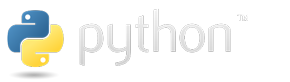
\includegraphics[width=0.4\textwidth]{Figuras/python-logo.png}
\caption{\label{fig:python-logo}Logo de Python}
\vspace*{-10pt}
\end{figure}

\subsection{Django}
Django es un framework web de alto nivel que permite el desarrollo rápido de sitios web seguros y mantenibles. Desarrollado por programadores experimentados, Django se encarga de gran parte de las complicaciones del desarrollo web, por lo que puedes concentrarte en escribir tu aplicación sin necesidad de reinventar la rueda. Es gratuito y de código abierto

\subsection{Bases de datos}
Para el desarrollo de la aplicación web se desplegaron dos bases de datos para poder aprovechar las caracteristicas de los datos y flujos involucrados:
\begin{itemize}
\item Una base de datos Postgresql para la gestión de los datos y elementos de la aplicación web en si misma.
\item Una base de datos InfluxDB para almacenamiento de la información registrada por la operación de los sensores y actuadores de los dispositvos IoT.
\end{itemize}

\subsubsection{Postgresql}
Es un sistema de gestión de bases de datos relacional orientado a objetos y de código abierto. Sus principales caracteristicas son:
\begin{itemize}
\item Alta concurrencia.
\item Amplia cantidad de tipos nativos.
\end{itemize}

\subsubsection{InfluxDB}
Es una base de datos de series temporales de código abierto desarrollada por InfluxData, utilizada para almacenar y recuperar datos de series temporales en áreas como monitoreo de operaciones, métricas de aplicaciones, datos de sensores de Internet de las Cosas y análisis en tiempo real. Está escrita en el lenguaje de programación Rust.

\subsection{Eclipse Mosquitto}
Eclipse Mosquitto es un broker de mensajes de código abierto que implementa las versiones 5.0, 3.1.1 y 3.1 del protocolo MQTT. Es ligero y adecuado para todos los dispositivos, desde computadoras de placa única de baja potencia hasta servidores completos. Esta escrito en el lenguaje de programación C.

\subsection{Grafana}
Grafana es una plataforma de visualización de código abierto que permite generar métricas, registros y trazas de datos de otras aplicaciones a través del uso de graficos y tablas organizados en dashboards. Permite consultar, visualizar, configurar alertas y comprender tus métricas, sin importar dónde se almacenen. 

\subsection{Node-Red}
Node-RED es una herramienta de programación que te permite conectar, integrar y automatizar dispositivos de hardware, APIs y servicios en línea. Su editor basado en paneles dentro del navegador facilita la creación de flujos mediante una amplia variedad de nodos, que luego se pueden implementar en su entorno de ejecución al mismo tiempo de manera sencilla.

\subsection{Docker}
Docker es una plataforma de código abierto que simplifica y automatiza el proceso de construir, desplegar y gestionar contenedores. Los contenedores son componentes estandarizados y ejecutables que combinan el código de la aplicación con las dependencias del sistema operativo.

\section{Adaptación del Marco Metodológico}
Para llevar a cabo la investigación propuesta, se decidió adaptar la metodología de forma que está favoreciera el desarrollo de los diversos elementos que se requerían. De esta manera se acordó hacer uso de lo siguiente:
\begin{itemize}
\item Sprints de dos semanas de duración.
\item Reuniones mensuales para realizar retrospectiva, sprint review y planificación de actividades para los siguientes sprints. Reunión en formato daily cada semana para comentar avances, bloqueos y recursos requeridos.  
\item Hacer entregas incrementales basadas en la adición de features y correcciones de código cada final de sprint.
\item Kick off del proyecto para el mes de septiembre del 2018.
\item Duración estimada del desarrollo de los dispositivos y de la aplicación web de 9 sprints (18 semanas).
\item El profesor Antonio Russoniello en calidad de tutor del trabajo especial de grado, asume el rol de Scrum Master. 
\item El bachiller Pedro Boll asume el desarrollo. 
\end{itemize}
Con ello definido, se presentan las siguientes actividades para el desarrollo y culminación del proyecto según los objetivos generales y especificos en la  tabla \ref{tabla:actividades_desarrollo}, junto con su duración aproximada.

\begin{table}[!htb]
\centering
\begin{tabular}{| m{4.5cm}| m{6.6cm}| m{3.2cm}|}
\hline
\multicolumn{3}{|c|}{Actividades de desarrollo} \\
\hline 
\centering Actividad & \centering Descripción & \centering Tiempo Estimado \tabularnewline \hline
1 & 2 & 3 \\ \hline
\end{tabular}
\caption{Actividades sugeridas para el desarrollo del trabajo especial de grado}
\label{tabla:actividades_desarrollo}
\end{table}
 